\chapter{Techniky, princípy a ciele útokov}
\label{kap:teoria}

V tejto kapitole uvedieme najčastejšie techniky používané na indukovanie chýb v hardvéri a vysvetlíme princípy týchto techník. Zároveň pre niektoré útoky zhrnieme existujúce výsledky popísané v iných prácach venovaných indukovaniu chýb.

Častým predpokladom úspešného útoku pomocou indukovania chýb je fyzický prístup k zariadeniu, ktoré je cieľom útoku \cite{lowcost}. Väčšina takýchto útokov vyžaduje miernu modifikáciu hardvéru, aby bolo možné ovplyvniť jeho činnosť, napríklad odstránenie niektorých komponentov, ktoré by mohli útok sťažiť, prípadne úplne znemožniť. Ideálnym scenárom pre útočníka je, ak môže komponent vybrať a prevádzkovať ho vo svojom prostredí. Aj preto sú častými obeťami takýchto útokov vnorené zariadenia \cite{lowcost}, väčšinou ovládané pomocou MCU (Micro Controller Unit, skrátene mikrokontrolér).

\section{Zmena napätia} \label{kap1:sek:zmenaNapatia}
Jednou z najjednoduchších a veľmi často využívaných techník indukovania chýb je zmena napätia, obvykle podpätie (angl. power glitch) \cite{crowbars, vccOnTheCheap, crypto}. Pre viac informácií o~indukovaní chýb technikou zmeny napätia odporúčame článok venujúci sa rôznym typom zmeny napätia \cite{powerGlitch}. Princíp takéhoto útoku spočíva v skonštruovaní obvodu, ktorý bude mať kontrolu nad napájaním zariadenia, na ktoré chceme útočiť a vo vhodných okamihoch na veľmi krátky čas (rádovo stovky nanosekúnd), vyvolá prudkú zmenu napätia. Takáto manipulácia môže spôsobiť nedefinované správanie na napájanom zariadení, najčastejšie možno očakávať, že ovplyvní aktívne časti hardvéru, napríklad obvody na procesore vykonávajúce jednotlivé inštrukcie. Častými symptómami takéhoto útoku sú napríklad preskočenie inštrukcie, nekorektné vyhodnotenie podmieneného skoku, chybný výsledok aritmetickej, či logickej operácie a pod. Najdôležitejšia časť takéhoto útoku je správne načasovanie a dĺžka intervalu zmeny napätia. Pokiaľ je tento interval zmeny napätia príliš dlhý (viac ako 2-3 mikrosekundy), je veľká pravdepodobnosť, že nastane fatálne zlyhanie a následný reštart zariadenia. Práve požadovaná presnosť časovania je parameter, ktorý výrazne vplýva na technickú náročnosť útoku.

Pre implementáciu útoku využívajúceho techniku zmeny napätia sú zvyčajne potrebné dve základné súčasti. Jednou je obvod, ktorý dokáže dynamicky manipulovať s~napájaním zariadenia, na ktoré cielime a druhým je generátor riadiacich signálov pre tento obvod, ktorý dokáže generovať impulzy s dostatočnou presnosťou. V závislosti od zložitosti a požadovaných parametrov týchto dvoch komponentov sa odvíjajú aj náklady a náročnosť takéhoto útoku. Napriek tomu v porovnaní s inými technikami zmena napätia patrí k menej náročným na implementáciu a je preto veľmi často používaná. 

Jednoduchou implementáciou takéhoto útoku môže byť napríklad použitie tranzistora, ktorým vieme spínať napájanie na mikrokontroléri. Takýmto spôsobom vieme na krátky okamih zatvorením tranzistora vyvolať podpätie na mikrokontroléri a jeho následným otvorením vrátiť napätie do bežného stavu. Tým môžeme vyvolať chybné vykonanie jednej alebo viacerých nasledujúcich inštrukcií \cite{vccOnTheCheap}.

Útok založený na podobnom, ale mierne zložitejšom princípe využíva tzv. \uv{Crowbars} obvod. Princíp takéhoto obvodu spočíva v tom, že zdroj napájania paralelne zapojíme cez tranzistor do skratu. Generovaním impulzov do tranzistora vieme na veľmi krátky čas (desiatky až stovky nanosekúnd) vyskratovať napájací zdroj, čím spôsobíme prudké zmeny v napätí na mikrokontroléri. Aby bolo možné presnejšie zacieliť na konkrétnu časť vykonávaného kódu bolo ovládanie tohto obvodu synchronizované s externými hodinami cieľového zariadenia, znázornené na obrázku \ref{obr:vccSync} \cite{crowbars}. Výhodou takéhoto zapojenia v porovnaní s odpájaním cez tranzistor je rýchlejší pokles napätia. Nevýhodou môže byť vysoké zaťaženie zdroja počas skratu a veľký prúd, ktorý potečie cez obvod vytvárajúci skrat. Na obrázku \ref{obr:vccScheme} sú pre porovnanie znázornené schémy oboch spomenutých obvodov pre manipuláciu napájania cieľového zariadenia.

\begin{figure}[!tbp]
  \centering
  \subfloat[Ovládanie tranzistorom]{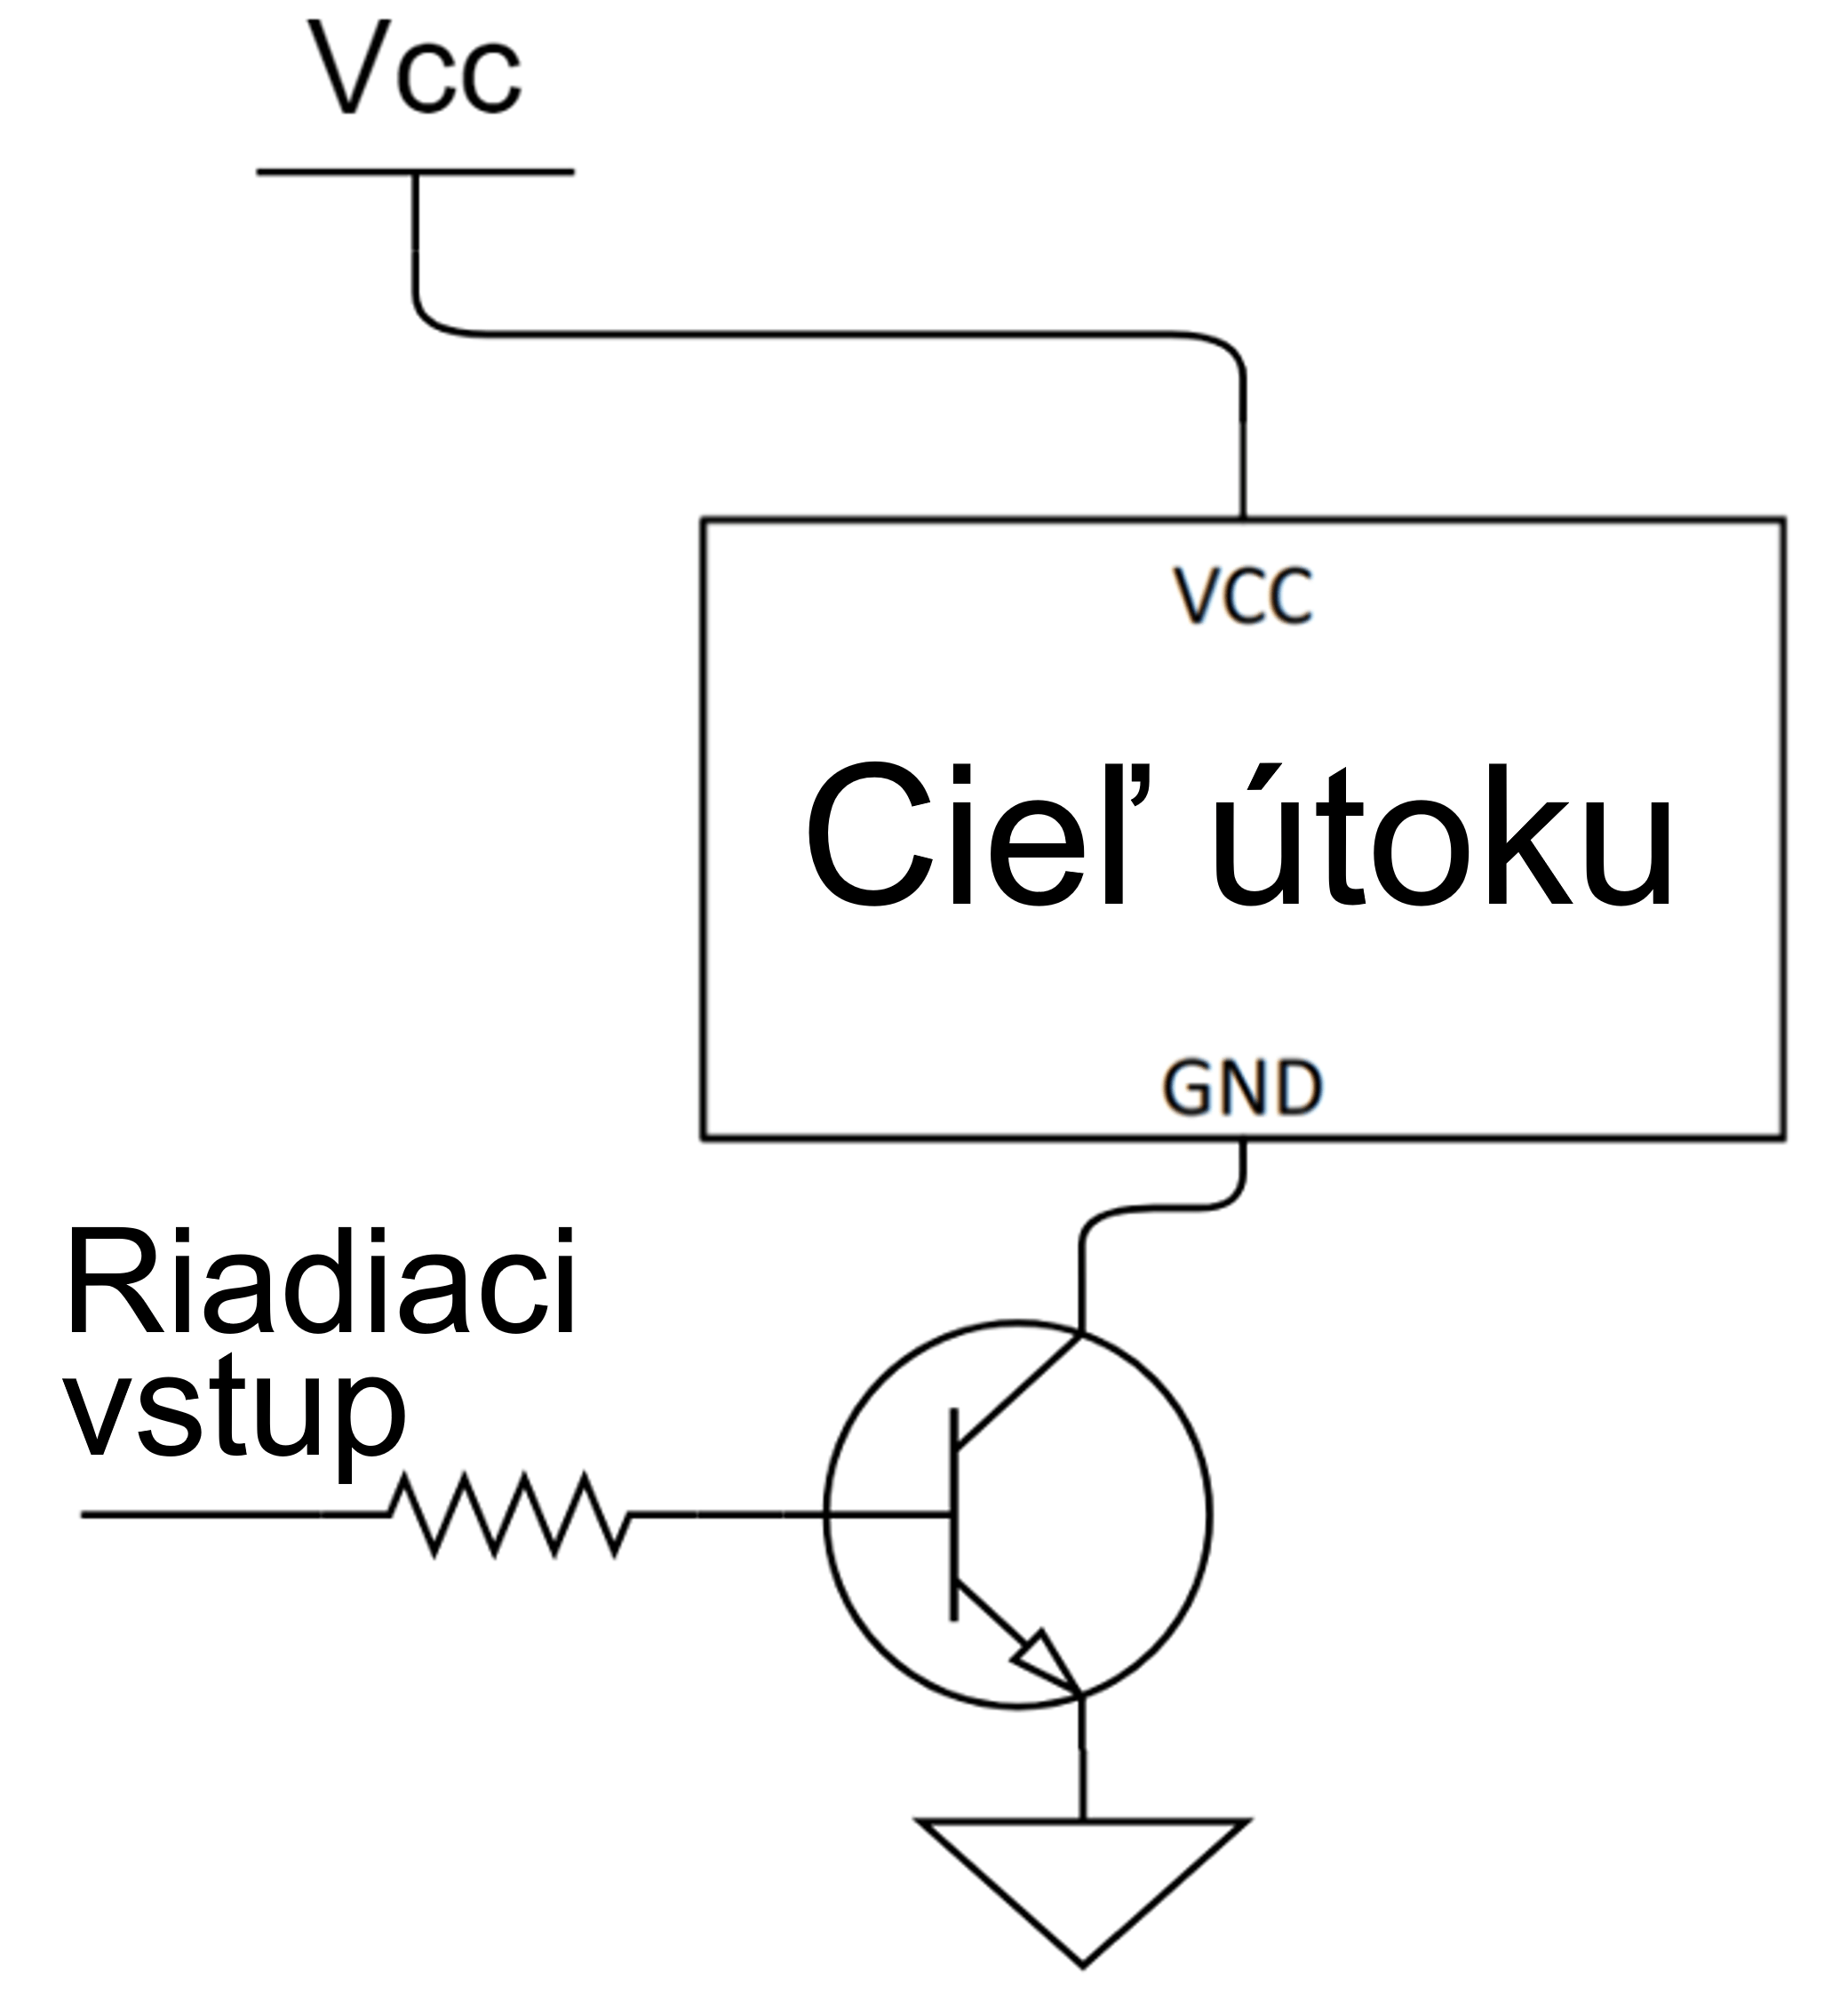
\includegraphics[width=0.3\textwidth]{images/transistor.png}\label{obr:vccSchemeA}}
  \hfill
  \subfloat[Skratovanie zdroja]{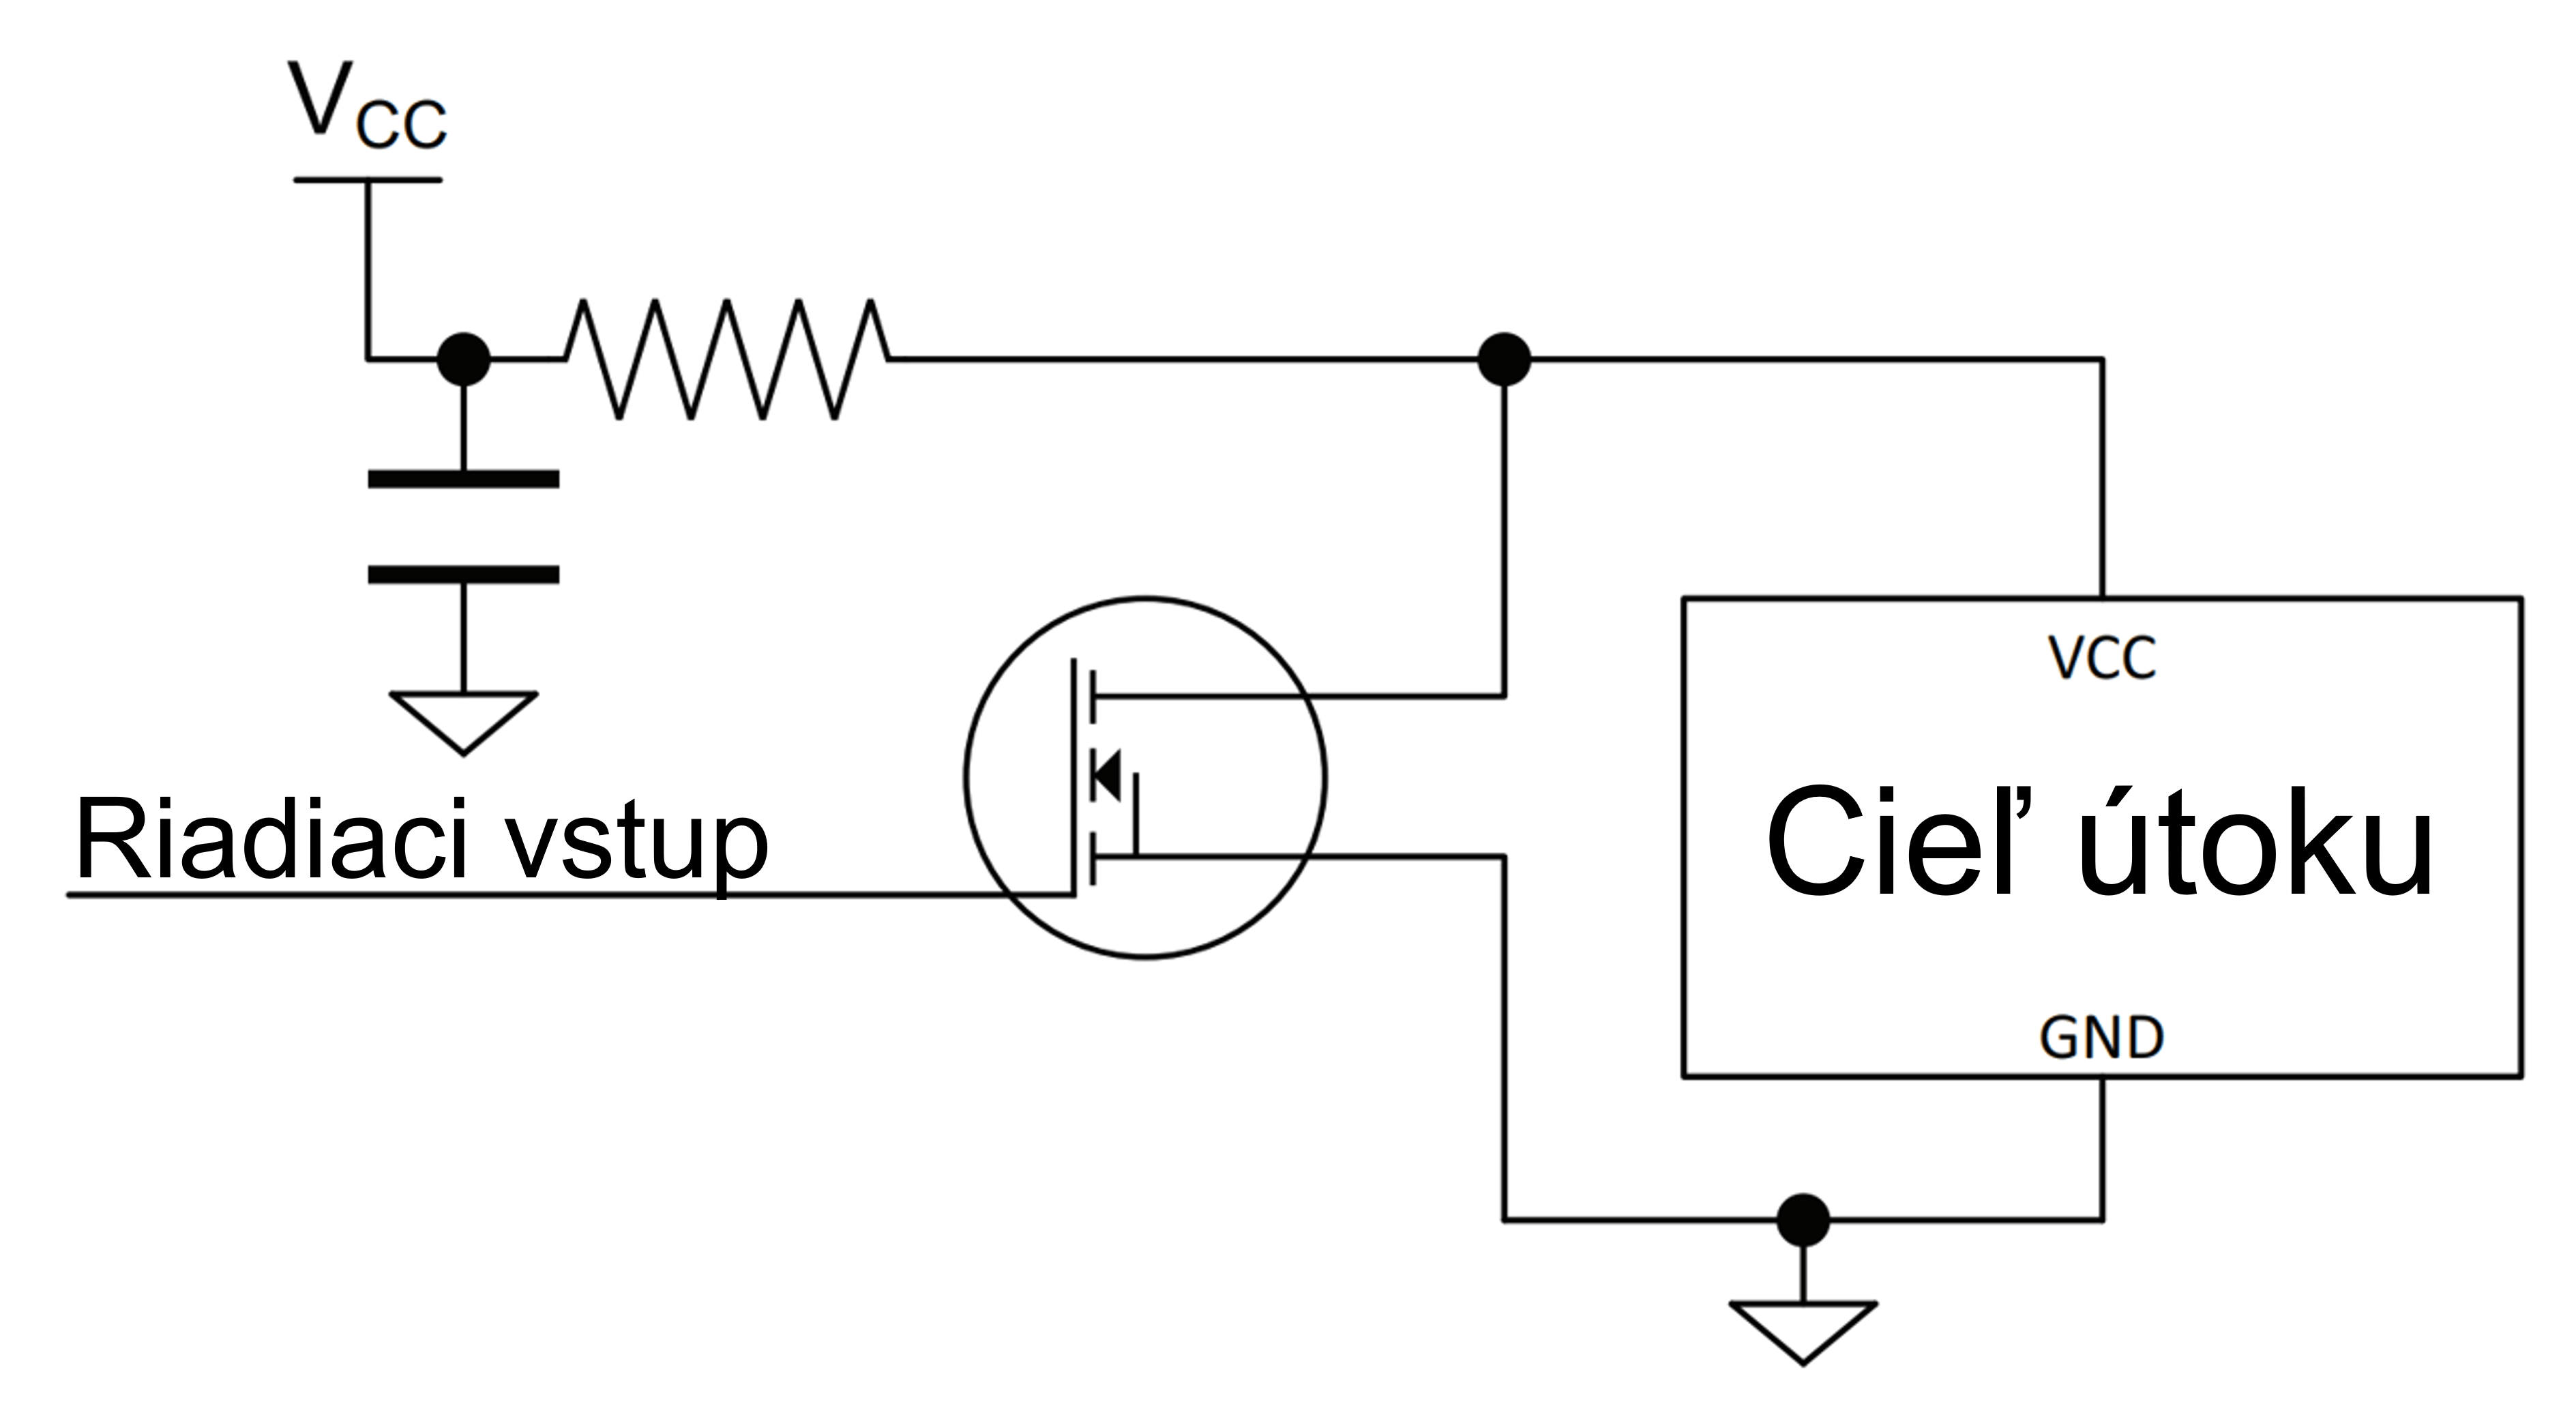
\includegraphics[width=0.5\textwidth]{images/crowbars.png}\label{obr:vccSchemeB}}
  \caption[Príklad obvodov pri útoku zmenou napätia]{Príklad obvodov pri útoku zmenou napätia. Obvod vľavo \ref{obr:vccSchemeA} ovláda napájanie cieľa pomocou tranzistora \cite{vccOnTheCheap}, vpravo \ref{obr:vccSchemeB} je obvod, pomocou ktorého možno skratovať napájací zdroj \cite{crowbars}.}
  \label{obr:vccScheme}
\end{figure}

\begin{figure}
    \centerline{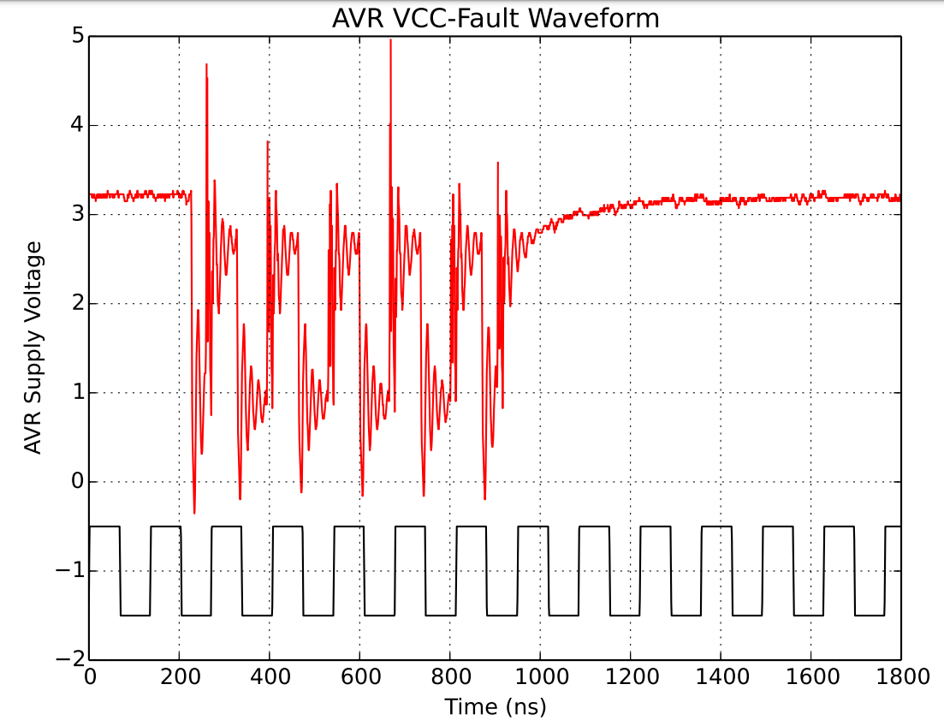
\includegraphics[width=0.5\textwidth]{images/vccSync.png}}
    \caption[Synchronizácia zmeny napätia s hodinami zariadenia]{Synchronizácia zmeny napätia s hodinami zariadenia. Červenou farbou je znázornená hodnota napätia v čase. V spodnej časti grafu (čierna farba) sú hodinové impulzy zariadenia \cite{crowbars}.}
    \label{obr:vccSync}
\end{figure}

Existujú rôzne spôsoby zapojenia, ktoré umožňujú meniť napätie na cieľovom zariadení. Líšia sa typom zmeny napätia, ktorý pomocou nich dosiahneme. Citlivejšie zariadenia by na úplné odpojenie napájania mohli zareagovať reštartom. Pri útoku na takéto zariadenia preto môže byť vhodnejšie vyvolať pokles napätia nie až na 0~V, ale napríklad na polovicu napájacieho napätia. V iných prípadoch môže byť potrebné vyvolať naopak prepätie na vyššiu hodnotu ako je napájacie napätie, prípadne tzv. zvonenie (angl. ringing) -- oscilovanie hodnoty napätia okolo úrovne napájacieho napätia.

Pre použitie týchto techník je dôležité zabezpečiť, exaktné časovanie generovaných riadiacich impulzov. To je možné zabezpečiť napríklad laboratórnym zdrojom alebo použitím špecializovaného hardvéru, napríklad open source platformy ChipWhisperer \cite{chipwhisperer}. ChipWhisperer integruje mnoho zariadení a obvodov používaných pri indukovaní chýb do jedného zariadenia a poskytuje ucelenú, voľne dostupnú skupinu nástrojov (angl. toolchain), pre zjednodušenie a automatizáciu jeho ovládania. Takéto zariadenia však môžu vyžadovať netriviálne náklady. Otázkou je, či aj lacnejšie riešenie, napríklad mikrokontrolér ATMega328P, ktorý je súčasťou populárnych vývojových dosiek Arduino, dokáže dosiahnuť rovnako dobré alebo aspoň porovnateľné výsledky. Jedným z cieľov tejto práce je práve vyskúšať takéto typy útokov pomocou mikrokontroléra ATMega328P.

\section{Manipulácia hodín} \label{kap1:sek:manipulaciaHodin}
Ďalšou často používanou technikou indukovania chýb je manipulácia impulzov prichádzajúcich z externých hodín do zariadenia (angl. clock glitch). Takouto manipuláciou možno vytvoriť nepravidelný taktovací signál, ktorý môže spôsobiť nekorektné správanie ním riadeného hardvéru. Riadiaca jednotka procesora na zariadení obvykle reaguje na nábehovú (niekedy dobehovú) hranu signálu prichádzajúceho od hodín zariadenia. Napríklad pridanie hrán do takto generovaného signálu môže mať za následok, že sa začne vykonávať ďalšia inštrukcia skôr ako sa predošlá inštrukcia stihla korektne dokončiť \cite{clock}. Správnym načasovaním tejto poruchy možno spôsobiť cielený efekt na program vykonávaný týmto hardvérom. Aby bol takýto útok úspešný je potrebné, aby bola riadiaca jednotka zariadenia priamo taktovaná externým oscilátorom. Napríklad niektoré zariadenia pomocou PLL (Phase Lock Loop) obvodu odvádzajú z prichádzajúceho externého signálu interný \cite{stmReference}, ktorý má rádovo vyššiu frekvenciu. Tento interný signál je následne použitý ako hodiny pre taktovanie procesora. Proti takýmto zariadeniam preto útok touto technikou pravdepodobne nebude účinný \cite{crowbars}.

Útok manipuláciou hodín môže byť realizovaný napríklad skonštruovaním kombinačného obvodu, ktorý pomocou logických hradiel, napríklad AND, OR a XOR, skladá rôzne výstupné signály zo vstupných. Vstupom do takéhoto obvodu môžu byť rôzne zdroje impulzov napríklad oscilátory s rôznymi frekvenciami, laboratórne zdroje, generátory signálov a ďalšie. Cieľom je rôznymi spôsobmi modulovať výstupný taktovací signál tak, aby v želaných okamihoch mal nesprávny tvar (nepravidelné takty, nesprávne hrany, vyššia frekvencia) a spôsobil tak poruchu na cieľovom zariadení. Pomocou logických hradiel možno vytvoriť rôzne vzorky signálu a následne napríklad využitím multiplexora automatizovane prepínať medzi jednotlivými výstupmi a tým dynamicky meniť výstupný hodinový signál. Na obrázku \ref{obr:clock} je znázornená ukážka schémy takéhoto obvodu \cite{clockCircuit}. Takýto obvod dokonca často nie je potrebné skonštruovať fyzicky, ale možno použiť aj programovateľné hradlové pole (FPGA), čo značne zjednoduší implementáciu útoku.

\begin{figure}
    \centerline{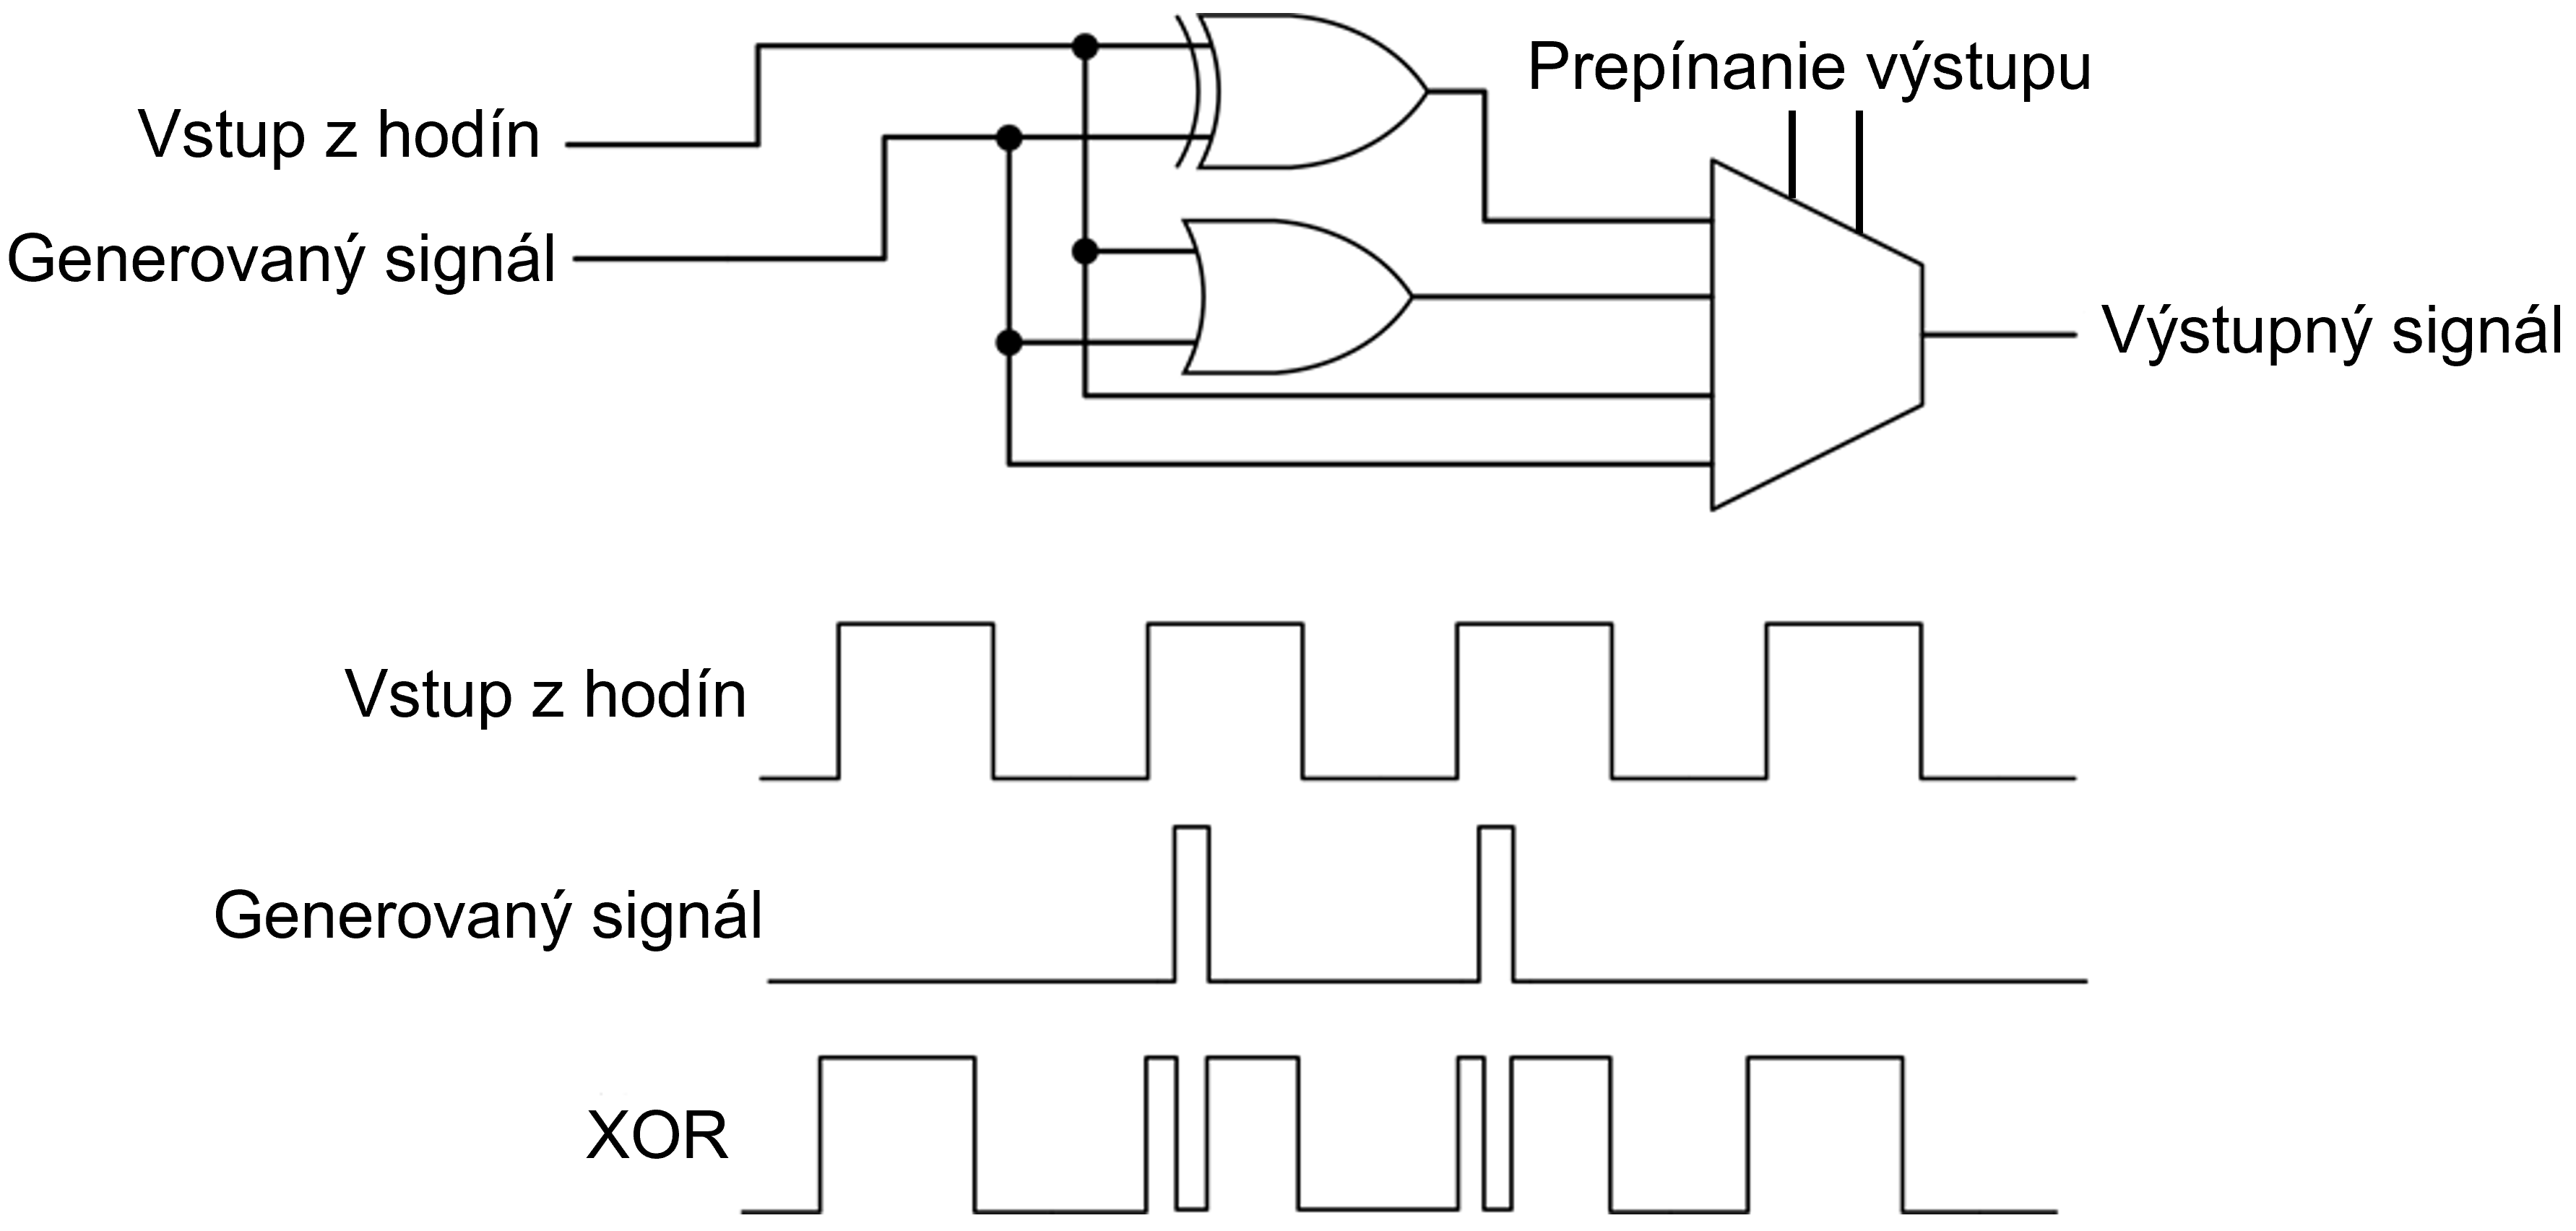
\includegraphics[width=0.75\textwidth]{images/clock.png}}
    \caption[Schéma obvodu pre generovanie nepravidelného signálu]{Schéma obvodu pre generovanie nepravidelného signálu. Vo vrchnej časti je znázornená schéma logického obvodu s multiplexorom, ktorým možno prepínať medzi výstupmi hradiel, v spodnej časti je príklad priebehu signálu na kanáloch multiplexora \cite{clockCircuit}.}
    \label{obr:clock}
\end{figure}

Poruchy, ktoré vieme touto technikou spôsobiť môžu byť rôzne, ale najčastejšie sa týkajú toku riadenia a dát, keďže hodiny generujú signál pre činnosť riadiacej jednotky procesora. Príkladmi takýchto porúch sú vynechanie inštrukcie, nekorektné načítanie dát z pamäte alebo nekorektný zápis do registra PC (Program Counter), čo môže spôsobiť nesprávny skok v rámci vykonávaného programu. Konkrétna implementácia takéhoto útoku na AVR mikrokontrolér z rodiny ATMega, do ktorej patrí aj nami zvolený ATMega328P (bližšie popísaný v kapitole \ref{kap:hardver}, sekcii \ref{kap2:sek:ATMega328P}) ukázala, že možno týmto spôsobom vyvolať viaceré z vyššie spomenutých porúch \cite{clock}.

\section{Elektromagnetické rušenie} \label{kap1:sek:elektromagnetickeRusenie}
Treťou známou technikou indukovania chýb je elektromagnetické rušenie alebo EMFI (Electromagnetic Fault Injection). Vplyvom elektromagnetického poľa možno narúšať fungovanie hardvéru na cieľovom zariadení a tým ovplyvňovať jeho činnosť. Takýto typ útokov zvyčajne vyžaduje dosku riadenú počítačom pohyblivú vo všetkých troch osiach (XYZ), pričom musí byť schopná s dostatočnou presnosťou nastaviť pozíciu antény, ktorá je zdrojom elektromagnetického rušenia. Generovaním impulzov do tejto antény v daných časových okamihoch možno spôsobovať želané rušenie \cite{emfi}.

Výhodou tejto techniky je možnosť s istou presnosťou (závisí od parametrov použitej elektroniky) útočiť na konkrétne časti obvodov na cieľovom čipe, napríklad pamäť, registre, či ALU. Nevýhodou je väčšia technická náročnosť útoku a obvykle drahší hardvér.

Sú známe aj ďalšie techniky indukovania chýb na hardvéri (napríklad laserové vypaľovanie), ktoré dokážu byť oveľa presnejšie a spoľahlivejšie. Ich implementácia je však oveľa náročnejšia, vyžaduje vysokú úroveň technickej zručnosti a veľmi vysoké finančné náklady \cite{laserFI}. Analýza týchto techník preto presahuje rámec tejto práce a nebudeme sa im podrobnejšie venovať.

\section{Ciele útokov} \label{kap1:sek:cieleUtokov}
Najčastejším cieľom útokov pomocou indukovania chýb je obídenie bezpečnostného mechanizmu. Príkladom je ovplyvnenie jednoduchej kontroly podmienky v programe vyvolaním chyby, ktorá spôsobí skočenie programu do nesprávnej vetvy, čo má efekt nesprávneho vyhodnotenia tejto podmienky. Zložitejšie útoky môžu cieliť na nesprávne vykonanie aritmetickej, či logickej operácie alebo nekorektné prečítanie dát z pamäte a~následne chybné rozhodnutie algoritmu, čo spôsobí cielené obídenie daného bezpečnostného mechanizmu. Cieľom takéhoto útoku môže byť získanie neoprávneného prístupu k službám alebo dátam zariadenia. Konkrétne napríklad prečítanie obsahu pamäte s~firmvérom aj pri zapnutej ochrane pred čítaním, útok na zavádzací softvér počítača, aby naštartoval systém z nepovoleného média a množstvo ďalších scenárov~\cite{AntiFI, bootloader}.

Ďalšia kategória cieľov týchto útokov sú zariadenia implementujúce kryptografické algoritmy. Tie sú často veľmi náchylné na implementačné chyby a preto dopady takýchto útokov môžu byť fatálne. Pomocou indukovania chýb možno napríklad prinútiť zariadenie, aby použilo nulový vektor ako kľúč pre symetrickú šifru. Potom už je jednoduché takto zašifrované dáta priamo dešifrovať. O niečo sofistikovanejšia, ale o~to účinnejšia, metóda útokov na kryptografické konštrukcie je tzv. DFA (Differential Fault Analysis). Princíp tejto metódy spočíva v indukovaní chýb v kryptografickom algoritme. Následne sa porovnávaním korektných a nekorektných výstupov určí aké inštrukcie a dáta sa v zariadení spracovávali. Takouto analýzou je možné napríklad zistiť použitý kľúč v symetrickej šifre alebo dokonca efektívne faktorizovať verejný modulus inštancie RSA schémy. Praktická úspešnosť týchto útokov bola demonštrovaná proti implementáciám schém AES a RSA na vnorených zariadeniach \cite{crypto}.

\section{Zranite\v{l}nosti a obranné mechanizmy} \label{kap1:sek:zranitelnostiAMechanizmy}
Samotná implementácia a následná úspešnosť útoku často závisí aj od samotného algoritmu, na ktorý je útok cielený, a spôsobu jeho implementácie od čoho sa odvíja ako veľmi môže byť náročná technická realizácia útoku. Niekedy nie je pre dosiahnutie cieleného efektu potrebné mieriť na jednu konkrétnu chúlostivú operáciu, ale stačí pokiaľ je výsledok série operácií nesprávny. Príkladom kódu, ktorý je náchylný voči chybám spôsobeným vplyvom prostredia je postupné inkrementovanie premennej v rámci cyklu, alebo séria viacerých priradení do rovnakej premennej počas výpočtu \cite{crowbars}. Kedy presne nastane chyba neovplyvní výsledný efekt útoku, za predpokladu, že chyba nespôsobí fatálne zlyhanie cieľového zariadenia. Pre tento typ útokov je často postačujúci lacný hardvér a nie je väčšinou potrebná synchronizácia zdroja chýb a cieľa \cite{crowbars, vccOnTheCheap}.

V iných prípadoch je potrebné cieliť na konkrétnu operáciu, čo zvyčajne vyžaduje vyššiu presnosť a synchronizáciu zariadení počas útoku. Príkladom takejto zraniteľnosti je zneužitie jednoduchej optimalizácie kompilátora \cite{AntiFI}. Kompilátor pri prekladaní cyklu, v ktorom sa postupne dekrementovala iterovaná premenná a postupne čítal vybraný úsek pamäte, použil inštrukciu BNE (Branch if Not Equal) miesto BLT (Branch if Less Than). Takáto optimalizácia je z teoretického pohľadu správna, keďže nemení význam algoritmu a test na nulu možno efektívnejšie vykonať ako všeobecné porovnanie. Keď v takto upravenom programe spôsobíme vynechanie tejto inštrukcie práve vtedy, keď má dôjsť k ukončeniu cyklu, dosiahneme tým, že takýto program bude pokračovať v cykle až kým nepretečie hodnota iterovanej premennej. Takýto útok bol demonštrovaný a autorovi sa podarilo prečítať firmvér na mikrokontroléri napriek tomu, že k nemu nemal mať prístup. V prípade, že by kompilátor použil inštrukciu BLT, bolo by potrebné pravidelne v každej iterácií spôsobiť takúto chybu, čo je pre útočníka náročnejšie \cite{AntiFI}.

Existuje viacero obranných mechanizmov, ktoré dokážu takéto útoky skomplikovať, niekedy až znemožniť. Medzi aktívne mechanizmy patrí detekcia takýchto útokov s využitím špecializovaného hardvéru, alebo softvéru a následne spustiť bezpečnostné opatrenie, napríklad reštart zariadenia. Aktívna detekcia útokov zvyšuje spotrebu zariadenia, čo najmä v prípade vnorených systémov môže byť hlavne pri napájaní z~batérie problematické riešenie. Jednoduchší, ale niekedy postačujúci, je pasívny spôsob obrany, napríklad úprava kódu tak, aby bol menej chúlostivý voči chybám \cite{AntiFI}. Pridanie náhodných oneskorení do programu môže sťažiť situáciu útočníkovi, ktorý potrebuje presne načasovať útok na konkrétnu operáciu \cite{AntiFI}. Ďalšími opatreniami môže byť nepoužívanie binárnych premenných pri vetvení programu a rovnako nepoužívanie triviálnych konštánt (0, súvislý vektor jednotiek). Nastavenie konkrétnej netriviálnej hodnoty (napríklad 0xAA, 0xB9) vplyvom chyby je náročnejšie, niekedy zanedbateľne nepravdepodobné a možno tak takémuto útoku zabrániť.